\section{Implementation}
To evaluate the approaches described in the previous chapter, concrete realization of an SDN
controller and data processing engine is needed. With Apache Flink, the data processing engine
constraint was already given. Besides that, a middleware software has to be implemented as a layer
between network and high level data engine. To achieve the project goals, a middleware has to be
implemented to connect low level network management via SDN controller and high level distribution
of the data processing tasks.

\subsection{SDN Controller}
In the open source community, there are some realizations of SDN controllers. The most popular ones
are POX/NOX, Floodlight and OpenDaylight. We use the de-facto standard OpenDaylight (ODL) as our SDN
Controller. It features good interoperability as well as scalability. It communicates via OpenFlow
with the virtual switches for routing and forwarding purposes as well as via a REST-interface with
custom programs, acting as a server providing network information on demand. 

\subsection{Requirements}
In the previous sections, two approaches have been introduced: Bottom Up and Top Down.
Implementation of the logic and algorithms relies on some requirements to the middleware software.
First, the middleware has to obtain information about the network topology and its current status.
To get information about the underlying network, a REST client is required to communicate with the
Northbound Topology API of OpenDaylight controller. Another requirement to the specification of the
middleware is realization of the scheduling approach. More specifically, it is about to implement an
algorithm of how the physical hosts (slots) are assigned to the tasks of the data processing engine.
This should be achieved in a way that the network communication between hosts is efficient and the
network resources are utilized as much as possible. The host assignment should be based on the
information about the network topology and the current status. The Top Down approach tries to
optimize the network utilization during runtime. The middleware needs to have information about the
currently executing job and its deployment (and distribution) in the network. This information is
provided by the data processing engine and should be transferred to the middleware. The middleware
has to analyze the data and optimize data flows by setting network flows through SDN controller. As
an optional requirement, a graphical representation of the current network topology and the host
assignment may be implemented. This functionality can be very useful for monitoring, controlling and
debugging of the middleware and the current job execution.

\subsection{Middleware Architecture}

\begin{figure}[h]
    \centering
    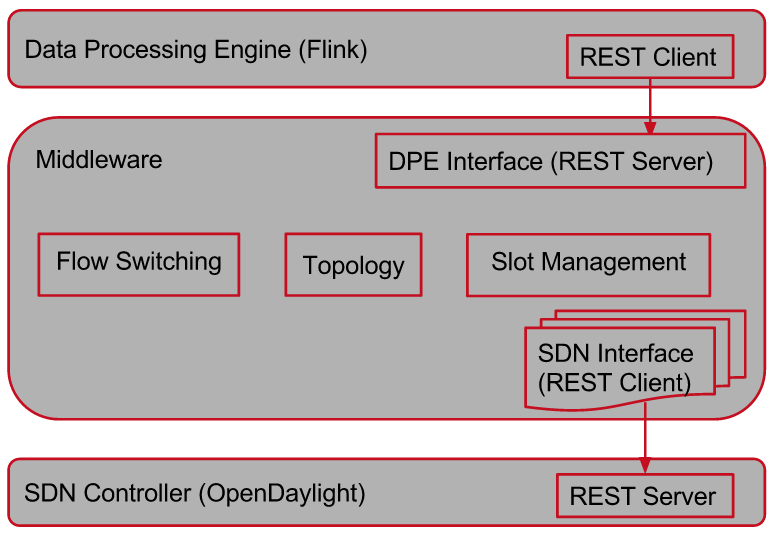
\includegraphics[width=0.8\textwidth]{graphics/architecture.png}
    \caption{Middleware Architecture}
    \label{fig:architecture}
\end{figure}

The architecture of the implemented middleware software is shown in Figure 3. The highest level in
the architecture is the data processing engine Flink. After the creation of the execution graph and
before deployment on the hosts, a communication-client has been implemented into the Flinks
scheduler-internals to communicate with the middleware. This client sends the execution graph and
requests new hosts for the job as soon as they are needed. The hosts, which finished execution are
released through a call of this client as well. The corresponding server side is a part of the
middleware. There are four other modules in the middleware. The topology module collects all the
data about the network: topology (network devices, hosts and connections between them) and the
current utilization of the network. The slot management part is responsible for slot allocation for
the distributed data engine. Algorithms behind it and the generic API belong to this module as well.
The flow switching module takes care about the optimization of the network flows based on the
current execution graph and network status. In order to access the Northbound API of the SDN
controller, generic interfaces were defined so that the middleware does not depend on one particular
implementation of a SDN controller. The concrete realization of northbound clients was done
separately for the required APIs, such as Flow Programmer and Topology API. A Module for network
visualization was implemented as well as part of the middleware. Technically, the middleware is
implemented as a Maven multi module project. This decision was made to take advantage of the
benefits of a structured project powered by a feature rich build system: flexibility,
customizability, dependency management, task automation and more. All the algorithms are covered
with tests and the source code is published under Apache License on the public repository hosting
service.
